%===================================== CHAP 2 =================================

\chapter{Prestudies}
\label{ch:prestudies}

\section{Customer input}
\label{sec:prestudies-customer_input}

In the first meeting with the customer, the group received input about the overall structure of the product, as well as the research required. The customer put emphasis on a few important factors when designing the application. The protocol implementation had to be modularized in such a way that additional protocol support could be added with ease at a later time. A graphical administration interface was also required, to be able to review broker data and adjust publisher/subscriber mappings. Additionally, extensive research had to be done, both to learn how the different protocols work, and to get an overview of the publish-subscribe pattern in general. These factors had an impact when choosing what sort of solution the group would develop. It also affected the development and research methodology.

The application was meant to be used internally by the Norwegian Armed Forces. Due to this, the group didn't have to consider the targeted user group in any way. The customer would field test the application at a later time. Thus, the only focus in that area was the feedback acquired from the customer.

\section{Publish-subscribe}
\label{sec:prestudies-publish_subscribe}

The implementation of the product had to be structured in a publish-subscribe messaging pattern. In standard messaging protocols, users send messages directly to other users or groups of users. Publish-subscribe is based on categories, and each message sent is placed in a specific category. Whenever a message is put in a category and sent, every subscriber on the category will receive the message. Publishers and subscribers are separated, as subscribers do not know which publishers, if any, exists. In the same manner, publishers have no insight into which, if any subscribers exists to the category. A user can be both a subscriber and publisher at the same time, depending on the category in question.

There are two main types of patterns used by the different protocols. The most popular one is using topics or queues. This method allows a subscriber to subscribe to a certain topic. Whenever someone posts a message in that topic, all subscribers on that topic receive the same message. Using queues, the idea is load balancing. The function of a topic queue is to allow for load balancing and to ensure that at least one subscriber gets the message. If no one subscribes to the topic a message is sent to, the message will be queued until someone does. Only one of the subscribers will get the message when queues are used. The other type of message subscription is using content filtering. Using this method, a subscriber will only receive a message if its contents match some given filtering criteria requested by the subscriber.

The general publish-subscribe pattern is visualized in this figure.

\begin{center}
  \begin{figure}[ht]
    \makebox[\textwidth]{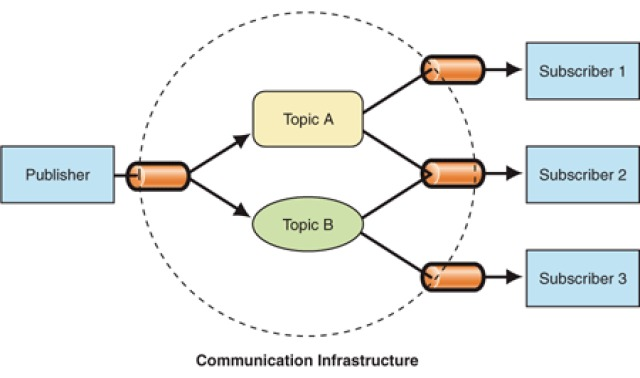
\includegraphics[width=0.7\textwidth]{fig/publish-subscribe.jpg}}
    \caption{Publish-subscribe}
    \label{fig:publish-subscribe}
  \end{figure}
\end{center}

\section{Protocols}
\label{prestudies-protocols}

The following sections describe the protocols the system were to support. The protocols are all based on publish-subscribe, but differ in their structure and implementation.

\subsection{Web Services Notification}
\label{subsec:prestudies-wsnotification}

WSN\footnote{\url{https://www.oasis-open.org/committees/wsn/}} is a messaging protocol developed by OASIS.\footnote{\url{https://www.oasis-open.org/}} It is a protocol that implements the publish-subscribe pattern over HTTP. The protocol uses SOAP to send XML messages over the network. The complete standard can be found here. \footnote{\url{http://docs.oasis-open.org/wsn/wsn-ws_base_notification-1.3-spec-os.htm}}

\subsection{Advanced Message Queing Protocol}
\label{subsec:prestudies-amqp}
AMQP\footnote{\url{http://www.amqp.org/}} is a binary protocol designed to send messages over a computer network. The protocol is built for handling the queuing of messages and routing (including publish-subscribe handling) in a reliable and secure way. The main funding and development of AMQP comes from the financial sector. The customer requested that version 1.0 of the AMQP protocol was to be implemented.

\subsubsection{AMQP version}
\label{subsec:prestudies-amqp-amqp_version}
AMQP has mainly two versions being used, with some substantial differences. 1.0, which is the current version, has fewer public implementations and less documentation and examples. 0.9.1 is radically different and does many things differently. As 1.0 was a requirement from the customer, little research was done on the difference between the versions of the standard. The important thing to note however, is the huge differences between the two. The developers of RabbitMQ(\ref{subsec:prestudies-existing_solutions-rabbitmq}), one of the most popular AMQP brokers states: "AMQP 1.0 is a completely different protocol than AMQP 0-9-1 and hence not a suitable replacement for the latter."

\subsubsection{Apache Qpid Proton}
To implement AMQP 1.0, the Apache Qpid Proton\footnote{\url{http://qpid.apache.org/proton/}} library was chosen. The Proton library is recommended by OASIS\footnote{\url{https://www.oasis-open.org}} as it provides language library bindings to over ten popular languages in addition to the native Java and C++ implementation. Proton was also chosen because of its wide use and the fact that it is actively maintained.

\subsection{Message Queue Telemetry Transport}
\label{subsec:prestudies-mqtt}
MQTT\footnote{\url{http://mqtt.org/}} is a publish-subscribe based protocol. It has the advantage of being lightweight and uses a minimal footprint wherever it can. The protocol also minimizes its use of bandwidth. MQTT has gained a lot of popularity over the last years, and its properties makes it suitable for everything from embedded system to big implementations like the Facebook Messenger\footnote{\url{https://www.facebook.com/notes/facebook-engineering/building-facebook-messenger/10150259350998920}}. This protocol was removed from the requirements in the mid stages of the project.

\section{Existing solutions}
\label{subsec:prestudies-existing_solutions}

Following is the evaluation of current existing solutions. These are products that partially covers the requirements, or could be used in the implementation in some way.

\subsection{Apache Apollo}
\label{subsec:prestudies-existing_solutions-apache_apollo}

Apache Apollo\footnote{\url{http://activemq.apache.org/apollo/}} is an open source project maintained by the Apache\footnote{\url{http://www.apache.org}} foundation and commercially supported by Red Hat \footnote{\url{http://www.redhat.com/}}. This application distinguishes itself from the existing solutions presented below, because it is a complete, protocol agnostic broker that translates freely between AMQP, MQTT, OpenWire\footnote{\url{http://activemq.apache.org/openwire.html}} and STOMP\footnote{\url{http://stomp.github.io}}. It is an up to date project, that is continually updated by the development team.

Apache Apollo can be considered the next generation of the older Apache ActiveMQ broker\footnote{\url{http://activemq.apache.org}}. It is a complete reimplementation of the old broker built on more modern programming concepts and has a more efficient message handler.    

\subsubsection{Evaluation}
\label{subsec:prestudies-existing_solutions-apache_apollo-evaluation}

Initially, the group set up an instance of Apache Apollo and read through both the user and developer documentation. Apollo seemed to be a very well written broker, and covered many of the requirements given by the customer.

The internals of the message queuing and message translation systems are well designed. It uses a non-blocking reactor thread model, which keeps all threads running and consumes tasks asynchronously, allowing for a fast message processing rate. Apollo dynamically converts large message queues from actual objects to pointer references when the queue becomes large. This helps mitigate the memory limits of the Java Virtual Machine, and allows Apollo to maintain queues larger than what a regular in-memory queue system would have. There was one issue with Apollo however. A lot of the functionality is written in Scala\footnote{\url{http://www.scala-lang.org/}}, which none of the group members had any prior experience with.

\subsection{RabbitMQ}
\label{subsec:prestudies-existing_solutions-rabbitmq}

RabbitMQ\footnote{\url{https://www.rabbitmq.com}} is an open source project created and maintained by Pivotal Software\footnote{\url{http://www.pivotal.io}}, which provides commercial support for the product. The software is mainly written for version 0.9 of AMQP, but supports version 1.0 via an experimental plug-in. There is also plug-in support for MQTT. RabbitMQ provides a large amount of bindings for a wide range of different programming languages. RabbitMQ and its plugins are written in the Erlang programming language\footnote{\url{http://www.erlang.org}}.

\subsubsection{Evaluation}
\label{subsec:prestudies-existing_solutions-rabbitmq-evaluation}

RabbitMQ and its plugins are implemented in a programming language and paradigm that was not preferred by the customer. Thus, it wouldn't be practical to build upon this solution. Additionally, no-one in the group had previous experience with Erlang. Therefore, the group concluded that further research was unnecessary.

\subsection{WS-Nu}
\label{subsec:prestudies-existing_solutions-ws_nu}

WS-Nu is a project developed as an assignment at NTNU. It is an implementation of the WSN protocol written in Java. It fully incorporates support for a large part of the WSN standard.

\subsubsection{Evaluation}
\label{subsec:prestudies-existing_solution-ws_nu-evaluation}

WS-Nu is a well written piece of software, which accomplishes many of the tasks of this project. Additionally, it was recommended for research and use by the customer.

\subsection{MicroWSN and NFFIPlayer}
\label{subsec:prestudies-existing_solutions-micro_wsn_and_nffiplayer}

MicroWSN and NFFIplayer are both software developed and provided by FFI. MicroWSN is an implementation of a WSN broker. NFFIPlayer is a graphical interface for testing MicroWSN. The package was created by FFI for testing in the field. However, the implementation is incomplete, and lacks several features that a complete implementation should have.

\subsubsection{Evaluation}
\label{subsec:prestudies-existing_solutions-micro_wsn_and_nffiplayer-evaluation}

The package was not considered for further development, due to its incompleteness, and that it is purely a broker for WSN. However, due to the graphical interface provided, it could be used to test the WSN implementation.

\section{Overall evaluation}
\label{sec:prestudies-overall_evaluation}

The main outcome of the prestudies phase, was the discovery of Apollo. It proved to be a solution it was possible to expand upon. One issue with Apollo, proved to be the massive code base. It was clear that it would be difficult to grasp, given the complexity and sheer size. A lot of the code was hard to understand, and lacked thorough documentation and community usage. Additionally, the web interface and a few core system components were built using Scala. Regardless, Apollo provided what seemed a very dynamic and robust implementation of both the AMQP and MQTT protocols, which were requirements of the customer. Expanding Apollo with WSN would be the best solution, as it would possibly open up time for adding other protocols the customer might want.

The group chose to introduce an extended research phase, in order to make a final decision regarding Apollo. This was based on an initial risk analysis of what would become a research project. These risks would lay the foundation of the research process, and define the different areas of focus. The risk analysis is shown below, and a more detailed description of the methodology is explained in section \ref{subsec:process_and_methodology-process-methodology-research}.

\begin{table}[ht!]
\centering
\resizebox{\textwidth}{!}{%
\begin{tabular}{|p{0.4\linewidth}
                |p{0.2\linewidth}
                |p{0.15\linewidth}
                |p{0.25\linewidth}|}
\hline
\rowcolor{lightgray}
\textbf{Description}                                 & \textbf{Likelihood (1-9)} & \textbf{Impact (1-9)} & \textbf{Importance (Likelihood * Impact)} \\ \hline
Apollo being too complex                    & 5                & 9            & 45               \\ \hline
Unable to learn Scala well enough           & 2                & 6            & 12               \\ \hline
Unable to implement additional modules      & 3                & 9            & 27               \\ \hline
Too much time required to implement WSN     & 4                & 9            & 36               \\ \hline
Difficulty in altering the Apollo admin interface & 4                & 7            & 28               \\ \hline
Apollo being incompatible with a protocol such as WSN  & 4                & 10            & 30               \\ \hline
\end{tabular}
}
\caption{Risk analysis for building the system based on Apollo}
\label{tab:risk_analysis_apollo}
\end{table}

\subsection{Alternate solution}
\label{subsec:prestudies-alternate_solution}

If the outcome of the research phase would result in discarding of Apollo as a foundation for the new system, a plan B was outlined. Plan B was to develop a completely new protocol brokering solution. WS-Nu would then be used as the WSN library of the product. 

The two major development tasks, were to create a web interface and the brokering solution in itself. The initial architecture outline was strongly influenced by the architecture of Apollo, due to its robustness and the sheer quality of the product. A quick draft was constructed to get an idea of the components needed to build a system from scratch. Influences from Apollo are the components in figure \ref{fig:arch_proposal} marked with green background color.

\begin{center}
  \begin{figure}[ht!]
    \makebox[\textwidth]{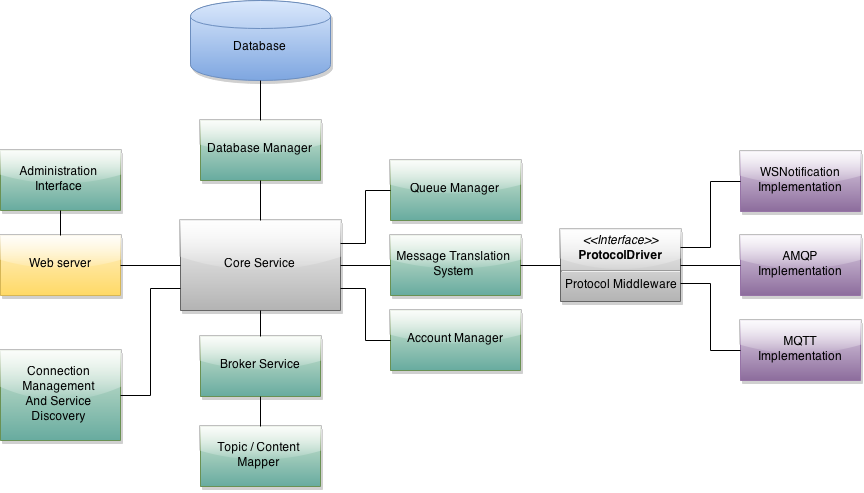
\includegraphics[width=\textwidth]{fig/arch_proposal_aleks.png}}
    \caption{Early Pub-Sub broker architecture influenced by Apollo}
    \label{fig:arch_proposal}
  \end{figure}
\end{center}

\subsection{Final decision}

After thorough research and consideration, the final choice fell on developing a new protocol brokering solution. Having no restrictions on namepolicy defined beforehand, the group eventually decided to name it OKSE(Overordnet kommunikasjonssystem for etterretning). The research work is more thoroughly documented in chapter \ref{subsec:process_and_methodology-process-methodology-research}, and the deciding factors are considered in chapter \ref{subsec:project_lifecycle-planning_and_research-research_phase-discussion}.

\section{Tools}
\label{sec:prestudies-tools}

Following is the list of all the tools used in the project. This includes tools used for communication, document sharing and development.

\subsection{Skype}
\label{subsec:prestudies-tools-skype}

Skype\footnote{\url{www.skype.com}} was the main tool used for communication with the customer. Meetings were held using the group call feature of Skype. Communication within the group was done using both group calls, as well as the instant messaging feature within Skype. The tool was convenient to use both for the customer and the group. It provided all the communication features needed, both voice communication and a textual chat.

\subsection{Mailinglist}
\label{subsec:prestudies-tools-mailinglist}

In addition to Skype, the group and the customer used email for communication between the meetings. To make sure that every group member always where up to speed on all relevant information, a mailinglist was created. The mailinglist was used to send a copy of every email received to the whole group. This was very beneficial as FFI only needed to communicate with one member and everyone got the information.

\subsection{Java}
\label{subsec:prestudies-tools-java}

The customer preferred that the main part of development was done with Java\footnote{\url{https://java.com/en/}}. Java is a programming language widely used in software development. The group chose version 8 as the target, which is the newest version. One of the main benefits of choosing Java and the Java Virtual Machine (hereby denoted as JVM) as the language and platform is that the broker could run on every system where JVM is available. This means that the broker would not be affected by different hardware architectures or operating systems as long as they are supported.

\subsection{Spring Framework}
\label{subsec:prestudies-tools-spring_mvc}

Spring Framework\footnote{\url{http://projects.spring.io/spring-boot/}} is a model view controller (hereby denoted as MVC) framework developed in Java. It is a modern framework mostly used for development of web-based applications. The framework was chosen after a quick evaluation of different possibilities. It was chosen because it was easy to learn, and provided exactly what was required, with a small amount of work to set up.

\subsection{Bootstrap}
\label{subsec:prestudies-tools-bootstrap}

Bootstrap\footnote{\url{http://getbootstrap.com/}} was chosen as a suitable framework for the visual aspects of the web application. The framework provided a large set of tools for page layout and elements, such as buttons, text and textfields. Designing it from scratch would have taken a lot of time, and was less important than the broker solution and the functionality of the web application. Thus, the framework seemed like an appropriate tool for its purpose.

\subsection{JavaDoc}
\label{subsec:prestudies-tools-javadoc}

In this project, the group chose to use JavaDoc, an automatic, comment based documentation tool to provide developer documentation of the code base. JavaDoc is supported in most Java Integrated Development Environments (hereby denoted as IDE), and allows for easy generation and updating of developer documentation. JavaDoc is the standard documentation tool for development in Java. Few good alternatives exist that covers the same functionality, and the tool was an obvious choice in this project.

\subsection{IntelliJ IDEA}
\label{subsec:prestudies-tools-intellij_idea}

IntelliJ IDEA\footnote{\url{www.jetbrains.com/idea/}} is a Java IDE. It contains a wide array of useful built-in functions for development in Java. It also includes support for build systems like Maven\footnote{\url{http://maven.apache.org/}} and Gradle\footnote{\url{https://gradle.org}}. Version control systems are also well integrated in the tool.

There exists many different development environments. Everything from simple text editors, to fully integrated development environments might be used. Considering development in Java however, one achieves some advantages by using a big platform. Both code completion, and functions for compiling code in the environment, makes the development process easier and faster. The group considered mainly three alternatives when evaluating the environment. IntelliJ, Eclipse\footnote{\url{www.eclipse.org}} and Netbeans\footnote{\url{www.netbeans.org}}. The choice came down to mainly two deciding factors. Both eclipse and Netbeans suffer from having a confusing amount of plugins for different tasks, where as the built in features of IntelliJ are widely cohesive. Secondly, IntelliJ was the first to release support for Java 8, and has proven to be stable and efficient over time.

\subsection{Apache Maven}
\label{subsec:prestudies-tools-apache_maven}

Apache Maven\footnote{\url{http://maven.apache.org/}} is a software solution for handling structuring, building and testing of Java projects. Maven also provides the developers with a package manager, which can be used to fetch libraries and add them automatically to the system. It is well implemented and widely used. Most Java Development Environments like Eclipse and IntelliJ supports Maven integration.

\subsection{TestNG}
\label{subsec:prestudies-tools-testng}

TestNG\footnote{\url{www.testng.org}} is a framework used for writing unit tests in Java. Compared to the more commonly used JUnit\footnote{\url{http://junit.org}}, TestNG is implemented with better handling of tests that requires threads, easier parametrized tests and the ability to more efficiently use data providers in the tests. TestNG also integrates out of the box with both Maven and Intellj IDEA.

\subsection{Git}
\label{subsec:prestudies-tools-git}

Version control is important when working on mid and large scale development projects. The group chose to use Git\footnote{\url{http://en.wikipedia.org/wiki/Git_(software)}} in collaboration with GitHub\footnote{\url{www.github.com)}}, a cloud hosted, distributed revision control system that allows all team members to access the code. Git provides complete history and version control, with complete offline support, as the Git working directory acts as a complete repository.

There are other distributed version control systems (hereby denoted as DVCS) available. However, the whole group had experience with both Git and GitHub beforehand, and the group agreed that using these services would be the best choice. Additionally, it would have been counterproductive to research and learn a different version control system. As most of the DVCS accomplishes the same tasks, the time should rather be spent on research and development.

% Someone please read if engrish makes sense.
\subsection{Jenkins}
\label{subsec:prestudies-tools-jenkins}

Jenkins\footnote{\url{http://jenkins-ci.org/}} is an open source continuous integration tool. It serves as a tool to automatize testing, maintenance and deployment. Whenever a change is integrated, Jenkins both runs tests and reports test results, as well as deploys the changes automatically.

Jenkins was used as an automatic test running tool, with full reporting from each build. It also automatically deployed the latest stable release of the system to the test server. Automatic test runs or deployment was triggered by integrating Jenkins with GitHub. Jenkins also provided out of the box integration with Maven and TestNG.

\subsection{Gantt project}
\label{subsec:prestudies-tools-gantt_project}

Gantt project\footnote{\url{http://www.ganttproject.biz/}} is a tool used to create gantt charts. It is a simple chart creation tool exclusively made for creating clean and structured gantt diagrams. The group had prior experience with the tool, and was chosen based on that.

\subsection{Google Drive}
\label{subsec:prestudies-tools-google_drive}

Google Drive\footnote{\url{https://drive.google.com/}} is a platform for sharing documents. Drive supports all necessary types of files, as well as support for real time cooperation on documents. The simplicity of Drive is what makes it an attractive platform. The ability to simply upload a file to the website, and instantly having it shared is both efficient and easy to grasp. Compared to using email for file sharing, or storage on a physical medium, a cloud solution seemed more suitable. 

Drive was used to share all text and image files used in the report. It also served as the main platform for sharing and collaborating on time-tables and agendas for meetings.

\subsection{LaTeX\ and ShareLatex}
\label{subsec:prestudies-tools-latex_and_sharelatex}

ShareLatex\footnote{\url{http://sharelatex.com}} is an online platform for collaborative editing of LaTeX documents. Furthermore, LaTeX is a typesetting system, designed for production of technical and scientific documentation.

LaTeX was chosen as the typesetting system for the report. Compared to other solutions like Microsoft Word, it allows you to generate clean and well formed documents. It also opens the opportunity for automatically generating a front page and table of contents. In the end however, the choice fell on LaTeX due to it being better, and more professional looking than many of it's alternatives.

ShareLatex can in some ways be compared to Google Drive. The difference is that it is exclusively built for sharing LaTeX documents. It features the ability to cooperate on documents in real time, as well as compile and preview documents.

\section{Risk analysis}
\label{sec:prestudies-risk_analysis}

The risk assessment was made early in the planning phase. The table (fig. \ref{fig:risk_analysis}) shows what was considered to be the most likely events happening, as well as preventive actions. Upon inspection of each of the risks, a number between 1 and 10 was chosen for the likelihood of the case happening, as well as the potential impact it would have. The final rank of the risk was defined as these two numbers multiplied. When a risk was identified, a remedial action was included, in order to reduce the potential impact it would have.

\small
\begin{longtable}{@{\extracolsep{\fill}}|p{0.13\linewidth}
                |p{0.11\linewidth}
                |p{0.08\linewidth}
                |p{0.12\linewidth}
                |p{0.2\linewidth}
                |p{0.2\linewidth}|@{}}
\hline
\rowcolor{lightgray}
\textbf{Description}                                 & \textbf{Likelihood (1-9)} & \textbf{Impact (1-9)} & \textbf{Importance (Likelihood * Impact)} & \textbf{Preventive Action}    & \textbf{Remedial Action} \\ \hline

Delivering an unsatisfying product.  & 3 & 9 & 27 & Frequent customer meetings. Have a mutual understanding of the goal of the project. & Document what went wrong, and why it happened.  \\ \hline

Too little work capacity within the development team & 5 & 5 & 25 & Frequent reviews of the progress. Proper distribution of workload. & Reviewing the time schedule. Add extra work hours each week. \\ \hline

Choosing a wrong/too complex architectural design. & 4 & 6 & 24 & Comprehensive research and planning. Set a deadline on which a final decision must be made on design approach. Constitute an alternative solution. & Fall back to alternate solution within the deadline. \\ \hline

Long term illness $>$ 3 days & 3 & 6 & 18 & Tell the group immediately when you notice illness etc. & In case of severe illness, negotiate with customer and supervisor about ambitions and requirements of the project. \\ \hline

Cooperation issues with the customer. & 3 & 5 & 15 & Frequent meetings with the customer. Uphold meeting agendas, and ensure mutual understanding at the end of meeting. & Emergency meeting with customer, assess and find a solution to the issue. \\ \hline

Customer does significant changes to the requirements. & 2 & 7 & 14 & Clearly define project scope and boundaries early on. & Negotiate with customer in order to find realistic goals. \\ \hline

Unable to meet time limit for deliverables. & 2 & 7 & 14 & Uphold time schedule. Review progress during meetings. & Working extra hours during evenings. \\ \hline 

Too little domain knowledge within the development team. & 7 & 2 & 14 & Proper planning and research. Continuous research and customer cooperation throughout the process. & Meetings with the goal of cooperatively gathering domain knowledge. \\ \hline

Data integrity (working on different versions). & 7 & 2 & 14 & Use a version control system. & Roll back to a state without conflicts. \\ \hline

Short term leave of absence. & 6 & 2 & 12 & Tell the group immediately when you are aware of leave of absence. & Distribute workload among the other members of the group. \\ \hline

Cooperation issues within the group. & 4 & 3 & 12 & Define each members role in the group. Find solutions to problems early. & Talk about the problems as a group, attempt to find a solution all parties agree on. \\ \hline

Data availability/loss. & 1 & 9 & 9 & Cloud storage, local backup on several devices. & Cooperate to assess damage, redo lost work. \\ \hline

Other subjects occupying work time. & 8 & 1 & 8 & Create a time table. Separate project work from other work. & Extra work time during evenings. \\ \hline

\caption{Risk analysis}
\label{fig:risk_analysis}
\end{longtable}
\normalsize

\clearpage